\documentclass[11pt]{article}
\usepackage{colacl}
\usepackage{natbib}
\usepackage{hyperref}
\usepackage{url}
\bibliographystyle{abbrvnat}
\setcitestyle{authoryear,open={(},close={)}}
\usepackage{graphicx}
\sloppy

\title{Cluster and Cloud Computing - HPC Twitter Processing}
\author{Adam Mooy\\
	    University of Melbourne\\
	    {\tt hmooy@student.unimelb.edu.au}
  \And Vinh Nguyen\\
  	University of Melbourne\\
	    {\tt vinh@student.unimelb.edu.au}}


\begin{document}
\maketitle

\section{Objective}

The goal of this assignment is to implement a simple, parallelise application leveraging the University of Melbourne High-Performance Computing (HPC) facility SPARTAN. The application will be used on a large Twitter data set to identify the top 10 most commonly used hashtags and most commonly used languages.

\section{Twitter Data Set}
The big twitter dataset comes in JSON format and has 4057522 rows of tweets from Sydney with a size of 19.34 GB. Every Tweet object\footnote{a.k.a Tweet Data Dictionary} includes an \textit{entities} section and a \textit{lang} section which provide metadata such as hashtags and language respectively. We decided to extract and count this readily available metadata. 

\section{Application details}
\subsection{Single process operation}
Every process is committed to a unique equal-size chunk of the large data file based on its rank. This assignment is achieved by instructing the process to compute the start and end byte positions for itself, following these equations
\[\textrm{start} =  \frac{\textrm{rank} \times \textrm{filesize}}{\textrm{number of processes}} \] 
\[\textrm{end} =  \frac{(\textrm{rank}+1) \times \textrm{filesize}}{\textrm{number of processes}} \] 

All processes read their assigned chunks line by line. Every input line is first removed of any unwanted trailing characters like ',' ']' before being parsed into a dictionary that contains the information of our interest. Specifically, the hashtag texts and the name of the language used in a tweet can be found by looking into the fields \textit{hashtags} and \textit{lang}, in the same order. Each process then updates its counts for each hashtag and language accordingly. 

\subsection{Parallel processing}
The single process design allows for a high level of independence between the parallel processes. In fact, there is no need for communication between the processes until they have all finalized their counts for each hashtag and language. Only then these counts are sent to Rank 0, where they are added together with their counterparts, to reveal the top 10 most common hashtags and languages.

\subsection{Invocation}

For job submission, the user needs to run the following shell command:
\begin{flushleft}
\t sbatch {-}-nodes=\$nodes {-}-ntasks=\$ntasks {-}-time=\$time {-}-export=ALL,DATAFILE=\$file\\ {-}-output=results/\$\{nodes\}n\$\{ntasks\}c-\\\$\{file\#\#*/\}-\%j.out \$script
\end{flushleft}
with the pre-defined variables: \$nodes = number of nodes (e.g 1), \$ntasks = number of tasks (e.g 8), \$time = time limit for job (e.g 00:02:00), \$file = path to data file (e.g /data/projects/COMP90024/bigTwitter.json), \$script = path to job script (job.slurm).

Inside the slurm script, our application is invoked via the \t srun command. Output files are stored in the existing folder 'results', named after the number of nodes, number of tasks and the data filename that we have used.

\section{Experiment}

Theoretically, Cloud nodes are comparatively slower, especially on multiple node jobs because the communication between Cloud nodes is slower than Physical nodes. In contrast, Physical nodes are connected by high-speed 25GB networking with 1.15 µsec latency which is preferable for multi-node jobs. When experimenting on small and tiny twitter files, Cloud partition execution time is faster than Physical partition. The reason could be the traffic was not too intense; therefore, it has lower latency and outperforms Physical nodes.  However, since both small and tiny Twitter file sizes are relatively small compared to big Twitter, Physical partition is used when running application on the big Twitter file. In order to have a proper comparison, Intel(R) Xeon(R) Gold 6154 CPU @ 3.00GHz nodes were used.

We run our application in various modes in order to evaluate changes in performance (runtime) when there is a change in the number of tweets processed and computing resources (nodes and cores).

\begin{table}[h]
 \begin{center}
\begin{tabular}{|l|l|l|l|l|}

      \hline
       File & Tweets &1N1C & 1N8C & 2N8C  \\
      \hline\hline
      Tiny & 999 & 0.586s & 0.734s & 0.823s \\
      Small & 4999 & 1.092s & 2.1s & 1.4s \\
      Big & 4057522 & 13m37s & 1m43.6s & 1m45s \\

     \hline

\end{tabular}
\caption{Run-time on different resources across different amounts of tweets}\label{table1}
 \end{center}
\end{table}

\begin{figure}[h]
\centering
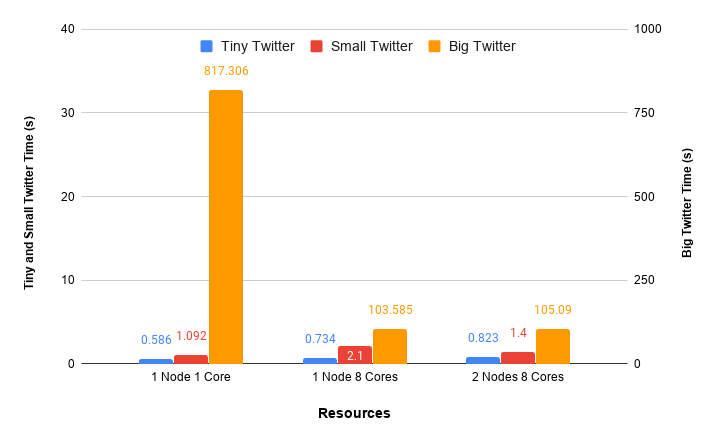
\includegraphics[width=7.5cm, height=7cm]{twitter_hashtags/report/chart.png}
\caption[Caption for LOF]{Execution time for twitter files under different resources\protect\footnotemark}

\end{figure}

Regardless of what resources we use, we also found the same results for the 10 most common hashtags and languages used in the big Twitter file (shown in Table 2 and 3). (Note that some languages other than English may not be displayed properly)

\begin{table}[h]
 \begin{center}
\begin{tabular}{|l|l|l|l|l|}

      \hline
      Rank &Hashtags & Counts   \\
      \hline\hline
      1 & auspol & 19878 \\
      2 & coronavirus & 10110 \\
      3 & มาพ่องเพิ่งอะไระไร & 7531 \\
      4 & firefightaustralia & 6812 \\
      5 & oldme & 6418 \\
      6 & sydney & 6196 \\
      7 & scottyfrommarketing & 5185\\
      8 & grammys & 5085 \\
      9 & assange & 4689 \\
      10 & sportsrorts & 4516 \\
    
     \hline

\end{tabular}
\caption{Top 10 most common hashtags}\label{table2}
 \end{center}
\end{table}


\begin{table}[h]
 \begin{center}
\begin{tabular}{|l|l|l|l|l|}

      \hline
      Rank &Languages & Counts   \\
      \hline\hline
      1 & English (en) & 3107115 \\
      2 & Undefined (un) & 252117 \\
      3 & Thai (th) & 134571 \\
      4 & Portuguese (pt) & 125858 \\
      5 & Spanish (es) & 74028 \\
      6 & Japanese (ja) & 49929 \\
      7 & Tagalog (tl) & 44560\\
      8 & Indonesian (in) & 42296 \\
      9 & French (fr) & 38098 \\
      10 & Arabic (ar) & 24501 \\
    
     \hline

\end{tabular}
\caption{Top 10 most common languages}\label{table3}
 \end{center}
\end{table}


\section{Discussion}
\subsection{Difference between file sizes}
The experiment (Figure 1) shows that the amount of time it takes to process a data file highly correlates with the number of tweets that file has, but not necessarily in a linear manner. For example, for 1 node 1 core the runtime ratio of the big Twitter file to the small file is in magnitude of hundreds, while that for 2 nodes 8 cores is not nearly a hundred. In other words, the amount of runtime declines at a higher rate than the increase in number of cores being used. This phenomenon may be a reflection of the fact that besides the actual processing time which can be optimized, there is also time required for communication between resources, which cannot be changed.

\subsection{Difference between computing resources}

Figure 1 shows the time spent to run the application under different resources. As expected the amount of time to run the application using 8 cores would be quicker than single-core. 2 Nodes 8 Cores is slightly slower than 1 Node 8 Cores because there is a communication time between 2 Nodes. 
\footnotetext{Results in output files 1n1c-bigTwitter.json-15909060.out, 1n8c-bigTwitter.json-15909058.out and 2n8c-bigTwitter.json-15909059.out slurm}
\newpage

\begin{table}[h]
 \begin{center}
\begin{tabular}{|l|l|l|l|l|}

      \hline
      Rank &1N1C & 1N8C & 2N8C  \\
      \hline\hline
      0 & 816.78 & 100.43 & 102.29 \\
      1 & - & 100.32 & 102.18 \\
      2 & - & 100.32 & 102.18 \\
      3 & - & 100.32 & 102.18 \\
      4 & - & 100.32 & 102.18 \\
      5 & - & 100.32 & 102.18 \\
      6 & - & 100.32 & 102.18 \\
      7 & - & 100.32 & 102.18 \\

     \hline

\end{tabular}
\caption{Execution time of each core}\label{table2}
 \end{center}
\end{table}

From Table 4, execution time on each core was recorded to ensure tasks were evenly distributed among all processes. Rank 0 took slightly longer as it had to gather all the counts from each process and compute the total count. 


\section{Conclusion}

This project demonstrated one of the main benefits of HPC supported by parallelization, which is the performance (speed). Although the procedure for requesting resources and submitting jobs are rather simple and highly automated for the user, a question may still remain regarding how we have the necessary resources distributed in order to maximize their usage. As we realize that there may be a significantly different consequence resulting from us choosing to utilize 2 nodes 8 cores instead of 1 nodes 8 cores (or vice versa), we need to make a conscious decision. For that matter, we opt for a less resource-centralized solution, where the total cores are evenly distributed over multiple nodes (rather than single node) for the reasons being higher fault tolerance and possible shorter queuing time. As a common logic, having all required computing resources spread over different places (nodes) makes our operation less vulnerable to system failure, apart from our request being easier to be granted.


\end{document}
